\documentclass{article}
\usepackage[utf8]{inputenc}
\usepackage{authblk}
\usepackage{setspace}
\usepackage{natbib}
\usepackage{hyperref}
\usepackage{graphicx}

\title{Zero-shot LLMs can save additional work in machine learning prioritised screening for systematic reviews}
\author[1,2]{Max Callaghan}

\affil[1]{Mercator Research Institute on Global Commons and Climate Change, Torgauer Straße 12-15, 10829 Berlin, Germany}
\affil[2]{%
	Potsdam Institute for Climate Impact Research (PIK), Member of the Leibniz Association, P.O. Box 60 12 03, 14412 Potsdam, Germany
}

\begin{document}
	\maketitle
	
	\doublespacing
	
	\begin{abstract}
		Zero shot learning using LLMs has received widespread attention in recent years, including in the automation of systematic review screening. 
		However, there has been insufficient research on robust processes to automate screening responsibly. 
		For systematic review screening, responsible automation requires that the risks of missing relevant studies (which are inherent when the process is automated) can be accurately quantified and managed.
		In this paper, we adapt LLM-assisted screening to the widespread machine learning prioritised screening paradigm, and use robust stopping criteria to quantify how much work can be responsibly saved with different levels of risk tolerance for missing studies.
		We find that that - even in the absence of detailed inclusion and exclusion criteria - LLM-assisted screening can save on average [x] percentage points of additional work compared to a baseline model.
		Across the whole database of [x] systematic review datasets, which would have required [x] hours to screen manually, LLM-assisted screening can reduce the time required to [x] hours, with the next best model reducing the time required to [y] hours, while still ensuring a 95\% chance of missing no more than 5\% of relevant studies.
	\end{abstract}

	\section*{Introduction}
	
	Systematic Reviews are important tools to synthesise findings across multiple studies, enabling decision-makers to make decisions that are informed by the best available evidence. 
	A key part of the process of systematic reviews involves finding studies using a transparent process that aims to be as comprehensive as possible. 
	Usually, bibliographic records are searched for using structured queries across multiple databases \cite{lefebvre_chapter_2023}.
	This results in a list of records that may or not be relevant to the review. The titles and abstracts of these records are then examined by hand - often by two independent reviewers - and it is judged whether they should be included, which means they are read again at the full text level, or excluded.
	This is a laborious and repetitive process - known as screening - and in times of increasing numbers of publications, this becomes more and more challenging. 
	
	There is a large literature \cite{omara-eves_using_2015}, going back nearly 20 years \cite{cohen_reducing_2006}, that investigates how machine learning might be used to automate parts of this process, in order to reduce the labour required to complete a systematic review. However, much of this literature demonstrates how one approach or another \textit{would have been able to} save work on past reviews where complete evaluation datasets are available, without showing how the approach could be used to \textit{responsibly} save work in new reviews where the inclusion and exclusion decisions are not known \textit{a priori}.
	
	This is reflected in the fact that the guidelines for conducting systematic reviews published by the Cochrane colloquium \cite{lefebvre_chapter_2023} do not recommend that machine learning is used to save labour during screening. This is because it remains uncertain how the use of automation may result in relevant studies being missed.
	
	Early attempts to automate systematic review screening used simple models like logistic regression and support vector machines. Lately, the literature on automating systematic reviews has increasingly turned its attention to the use of large language models (LLMs). However, not enough attention has been paid to comparing LLM-based approaches with the much simpler (and computationally less expensive) alternatives. Further, papers which have investigated the use of LLMs have so far not considered how they might be used in a responsible manner where evaluation data is not available.
	
	For example, in \cite{wang_zero-shot_2024}, the authors introduce a method to generate probability-like scores for the inclusion of each document, by retrieving the probabilities of the next token after prompting the model. The prompt gives information on the review and provides the title and abstract of the record in question, and asks the model to answer whether it should be included with a ``yes'' or a ``no''. The probability that the next token is ``no'' is subtracted from the probability that the next token is ``yes'', resulting in the inclusion score. This process has two advantages over simply prompting the model and recording whether it says yes or no. First, the result becomes deterministic, in that a single model will always give the same score for the same prompt. Second, in returning a probability-like score instead of a binary response, we are better able to discriminate between documents considered highly likely to be irrelevant and those considered mildly likely to be irrelevant by the model.
	
	However, the paper proposes a strategy to save work using the model that is not able to accurately quantify or mitigate the risk of missing studies. Documents with an inclusion score greater than a threshold paramater $\theta$ are screened by hand, while all remaining documents are automatically excluded. The methods proposed to set the threshold paramater (either extrapolating from other reviews, or by setting the paramater such that it achieves the desired recall level on a set of predefined relevant documents) are \textit{not} able to reliably ensure that a desired level of recall is met. 
	
	Although the LLM-based procedure is compared to a fine-tuned BERT-like model, the details of this are not clear, and it appears that there is no comparison to the most common mode of machine learning assisted screening, known as machine learning prioritised screening. With ML-prioritised screening, a subset of documents are screened by hand, and these documents are used to train a model to predict the relevance of remaining unscreened documents. A batch of those records with the highest predictions are then screened by hand, before the model is retrained using the expanded training dataset. This process continues until a ``stopping criterion'' \cite{SneydS19, callaghan_statistical_2020, lewis_confidence_2023} is met, which either aims to guarantee that a certain recall level has been met with a given confidence level, or which quantifies that the returns to additional screening are low. 
	
	In this paper, we adapt the probabilistic zero-shot screening process using LLMs to a ML-prioritised screening setting, and show that - when combined with statistically valid stopping criterion - it is able to reliably achieve high levels of recall while saving work. Secondly, we compare LLM-assisted approaches to simpler methods available, both in terms of the work saved, and in terms of computational requirements.
	
	\section*{Methods}
	
	\subsection*{Probabilistic inclusion scores from LLMs}
	
	Following \cite{wang_zero-shot_2024}, we write a prompt template (see supplementary material) that ``asks'' a large language model whether a document $d$ should be included in a review $t$. Instead of using the prompt to generate a response, we pass the prompt to the model and extract the next token probabilities. The inclusion score $S$ for document $d$ in review $t$ is given by subtracting the probability that the next token is ``no'' $P(no|d,t)$ from the probability that the next token is ``yes'' $P(yes|d,t)$.
	
	\begin{equation}S(d,t) = P(yes|d,t) - P(no|d,t)\end{equation}
	
	In a new review, one could generate scores in this way for each document returned by a query, and screen these in descending order of their inclusion score, applying a stopping criterion to decide when remaining unscreened documents can be excluded automatically.  We simulate this process using the Synergy dataset of completed reviews \cite{de_bruin_synergy_2023}, and report on the work that would have been saved, and the actual level of recall that would have been achieved, given a range of recall targets and uncertainty levels.
	
	We use the stopping criteria in \cite{callaghan_statistical_2020}\footnote{Using the python package available at \url{https://buscarpy.readthedocs.io/en/latest/}}, which uses the hypergeometric distribution to test a null hypothesis that a target level of recall has \textit{not} been achieved. When the 1 minus the p score returned by the criterion is below the our confidence level, which indicates that it would have been unlikely to observe the previous sequence of inclusion and exclusion decisions had we missed our recall target, screening is stopped. 
	
	\subsection*{Active learning baselines}
	
	With the LLM-assisted screening approach, predictions are made once for each document, and are made solely on the basis of the prompt. With active learning approaches, which are more commonly deployed, predictions are made using a model based on records that have already been screened, and the model is frequently retrained as more screening data becomes available, meaning that predictions are generated multiple times for many documents.
	
	We implement our active learning pipeline as follows for each model and each review dataset, where each dataset has $N$ unique documents. Screening here, in a simulation context, refers to revealing the screening decision that was made when the dataset was created.
	
	\begin{enumerate}
		\item ``Screen'' a sample of 10\% of papers in the review dataset. If no papers in the sample are relevant, keep screening until at least one relevant paper has been screened.
		\item Train the model using the screened documents and prediction inclusion for remaining unscreened documents
		\item Screen the $N/10$ documents with the highest predicted scores 
		\item Repeat steps 2 and 3 until all documents have been screened
	\end{enumerate}

	This process generates an ordered list of documents that corresponds to the order in which documents would have been seen if our approach was being applied in the real world. Using this ordered list, we calculate stopping points for a variety of recall targets and confidence levels.
	
	Because the random sample can affect the quality of the predictions and the resulting rankings, we repeat this experiment 100 times, each with a different random seed, for each model and dataset combination. 
	
	\section*{Results}
	
	\begin{figure}
		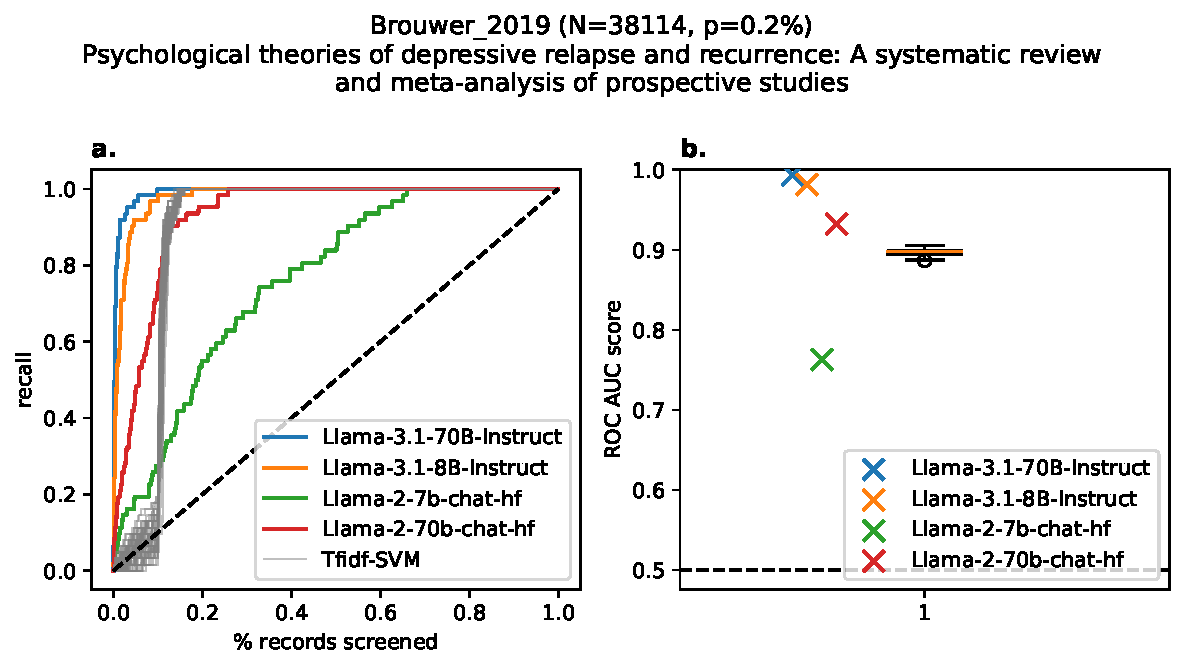
\includegraphics[width=\linewidth]{../../figures/Brouwer_2019.pdf}
		\caption{Rankings produced by LLM-assisted screening (coloured lines) and by active learning using a support vector machine. Left panel shows the recall achieved at different proportions of relevant documents screened. Right panel shows the distribution of ROC AUC scores for the support vector machine approach (boxplot) and for LLMs (coloured crosses)}
		\label{fig:rankings}
	\end{figure}
	
	First, we start by examining the rankings produced by our ML-assisted screening processes. Figure \ref{fig:rankings} shows these for a selected review dataset on Psychological theories of depressive relapse and recurrence, which contained 38,114 records, of which 0.2\% were relevant. Looking at the left side, we see that all evaluated models result in the identification of all relevant documents before all documents have been screened, meaning that work savings are in principle possible. On the right-hand side, we see the Receiver Operating Characteristic - Area Under the Curve (ROC-AUC) score, which measures the likelihood that a random relevant document is ranked higher than a random irrelevant record. A score of 1 indicates that all relevant documents are correctly identified first, before any irrelevant documents have been seen. A score of 0.5 indicates that the ranking is no better than chance.
	
	
	Overall, across the X datasets, Llama3.1 models achieves a higher ROC AUC score than the SVM baseline, while Llama2 models achieve a lower score (figure \ref{fig:macro}). Across both generations of Llama models, models with more parameters achieved higher scores than models with fewer paramaters. This difference was more pronounced for Llama2 than for Llama3.1 
	


	\begin{figure}
		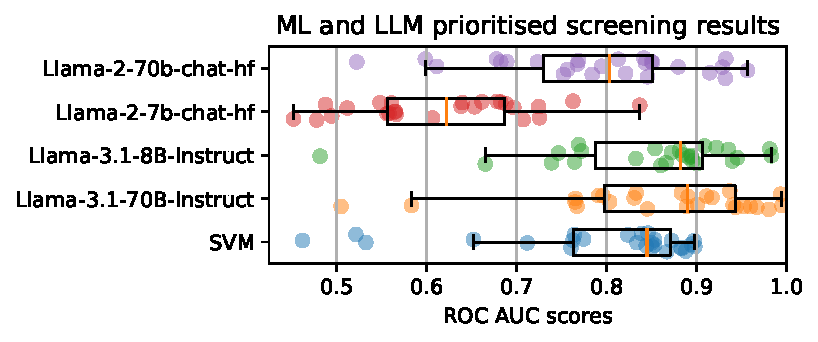
\includegraphics[width=\columnwidth]{../../figures/macro_comparison.pdf}
		\caption{The distribution of ROC AUC scores across datasets. The results for the support vector machine (SVM) display the median score for each dataset.}
		\label{fig:macro}
	\end{figure}
	
	\section*{Discussion}
	
	\bibliographystyle{unsrt}
	
	\bibliography{LLMs/stopping-criteria}
	%\bibliography{../LLMs}
	
	\appendix
	
	\section*{Supplementary Material}
	
	\subsection*{Prompt template}
	
	
\end{document}